\documentclass[a4paper]{llncs}

%%Allows the use of portuguese characters
\usepackage[utf8]{inputenc}
\usepackage[english]{babel}
%ensure that quoted texts are typeset according to the rules of your main language
\usepackage{csquotes}

%% Package to use images
\usepackage{graphicx}
\graphicspath{ {img/} }

\usepackage[printonlyused]{acronym}

%% References and stuff
\usepackage[backend=bibtex]{biblatex}
\bibliography{references}

%% Package used for quotations
\usepackage{csquotes}

% This adds numbering to subsubsections
\setcounter{secnumdepth}{5}

% This overrides the settings of the llncs class and displays the ToC
\setcounter{tocdepth}{3}

% This prevents the document title and the author from being part of the ToC
\makeatletter
\renewcommand*\l@author[2]{}
\renewcommand*\l@title[2]{}
\makeatletter

% Page format
%\usepackage{geometry}
%\geometry{
%	a4paper,         % or letterpaper
%	textwidth=15cm,  % llncs has 12.2cm
%	textheight=24cm, % llncs has 19.3cm
%	heightrounded,   % integer number of lines
%	hratio=1:1,      % horizontally centered
%	vratio=1:1,      % vertically centered
%}


\begin{document}

\title{Cooperative AI for Don't Starve Together}
\author{Fábio Vieira de Almeida}
\institute{Instituto Superior Técnico}
\thispagestyle{plain}
%\email{fabio.vieira.almeida@tecnico.ulisboa.pt}

\maketitle

\begin{abstract}
To be filled.
\end{abstract}

\tableofcontents
\newpage

\section{Introduction}

For games, one of the most important aspects is the player's experience.
The game's flow and immersion are key elements to this experience \cite{ijsselsteijn:userexperience}, and this is where \ac{AI} comes into play.

In the last years, in order to improve player's game play experience, the game industry have used \ac{AI} with several different purposes: player experience modelling, procedural content generation, massive-scale game data mining, and \ac{NPC} \ac{AI} \cite{yannakakis:gameairevisited}.

\begin{itemize}
	\item Talk about graphical believability and how AI in games should accompany this trend
	\item Talk about engagement in games through NPCs (better NPCs create a better game experience).
	\item Talk about the lack of AI for survival games (maybe use Left 4 Dead 2 as an example of an AI)
\end{itemize}

\subsection{Problem}
"Can we improve a player's gameplay experience in Don't Starve Together using social agents?"

\subsection{Hypothesis}


\subsection{Objectives}
Develop a model that combines the social interaction with players and the capacity of an agent to survive in a survival game
Check if players like to play with the agent
and check if they prefer to play with humans or the agent

\subsection{Document Outline}
\newpage
\section{Don't Starve Together}
\ac{DST} is a multiplayer wilderness survival game developed at Klei Entertainment, where the players must survive as long as they can.
The players must face the harshnesses of a procedurally generated world that is actively trying to kill them, either by cooperating or competing with each other.
Each game can last and indefinite amount of time which is only determined by the players' ability to survive, the better you play the game, the longer you can last.

Don't Starve Together, released on April 21st of 2016, is the standalone multiplayer expansion of the uncompromising wilderness survival game Don't Starve, also released by Klei on April 23rd of 2013 (check Fig. \ref{fig:don't-starve-together-poster}).
Both titles are available in several platforms ranging from PC's to consoles and even mobile devices.
By the end of 2013 the original title (Don't Starve) sold over one million copies and, currently, there are almost 3.5 million owners of the game only on Steam.
\ac{DST} counts with over 4.6 million owners on Steam and has a daily peak of concurrent players of well over 5 thousand, reaching as high as 9 thousand concurrent players.

\begin{figure}
  \centering
    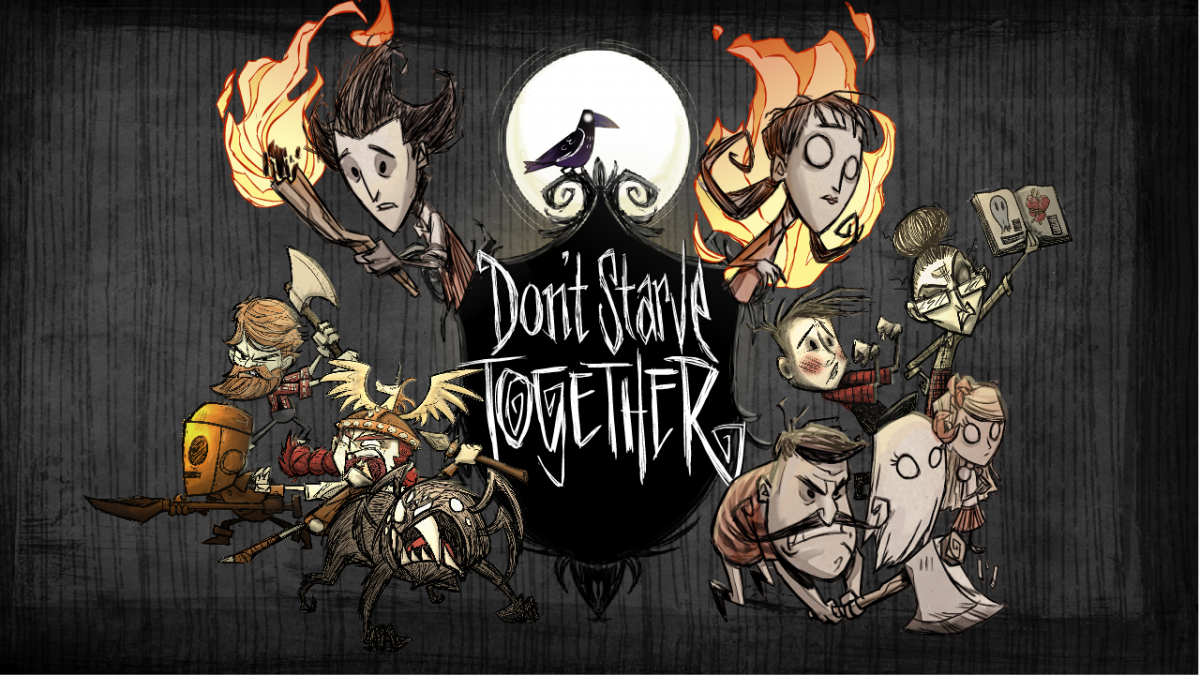
\includegraphics[width=\textwidth]{dont-starve-together-poster}
  \caption{Don't Starve Together poster with all original characters.}
  \label{fig:don't-starve-together-poster}
\end{figure}

The game counts with a developer maintained forum where there is an active participation in the forums by Klei Entertainment staff, which help in problem solving for community developed mods, bug fixing the game, and sharing development notes on the game.
Over twenty-five hundred mods are available for the game on the Steam Workshop, making \ac{DST} a well-suited option to implement and test our solution.

\subsection{The Game}
Before playing \ac{DST}, the players must first choose a character from a list of different characters.
Different characters have different characteristics and may be affected by the world in different ways (for example, WX-78 can eat spoiled food without penalties) and can even possess special items (such as Woodie's axe, \textit{Lucy the Axe}).
Upon entering the world, the player has nothing in its inventory (except for character specific items, as referred earlier) and thus needs to start collecting resources in order to survive.

During the game the player must pay attention to the three characteristics of his character: Hunger, Sanity, and Health.
The player dies (in \ac{DST} the player actually becomes a ghost that can be revived by other players or by finding a Touch Stone) once his Health reaches zero.
Both Hunger and Sanity can cause the player to loose Health (Sanity doesn't directly cause the player to loose Health, but the player will be attacked by creatures that appear due to the character's paranoia).

So, it is important for the player to keep Hunger, Sanity, and Health in check in order to survive.
The player will also need to take attention to the character's Wetness which is caused by rains.
Wetness will cause the items to loose efficiency and by using wet items the character will lose Sanity over time.
The player must also be aware of the temperature of his character as it can cause damage.
Both extreme hot and extreme cold will cause the player to continuously loose Health.

Taking care of the character's Hunger, Sanity, and Health is the players main concern during game play.
The player will accomplish this by collecting resources, crafting new items, cooking food, among other things (we will explore the player's possible actions in full detail further on).

\subsection{The World}

\begin{figure}
  \centering
    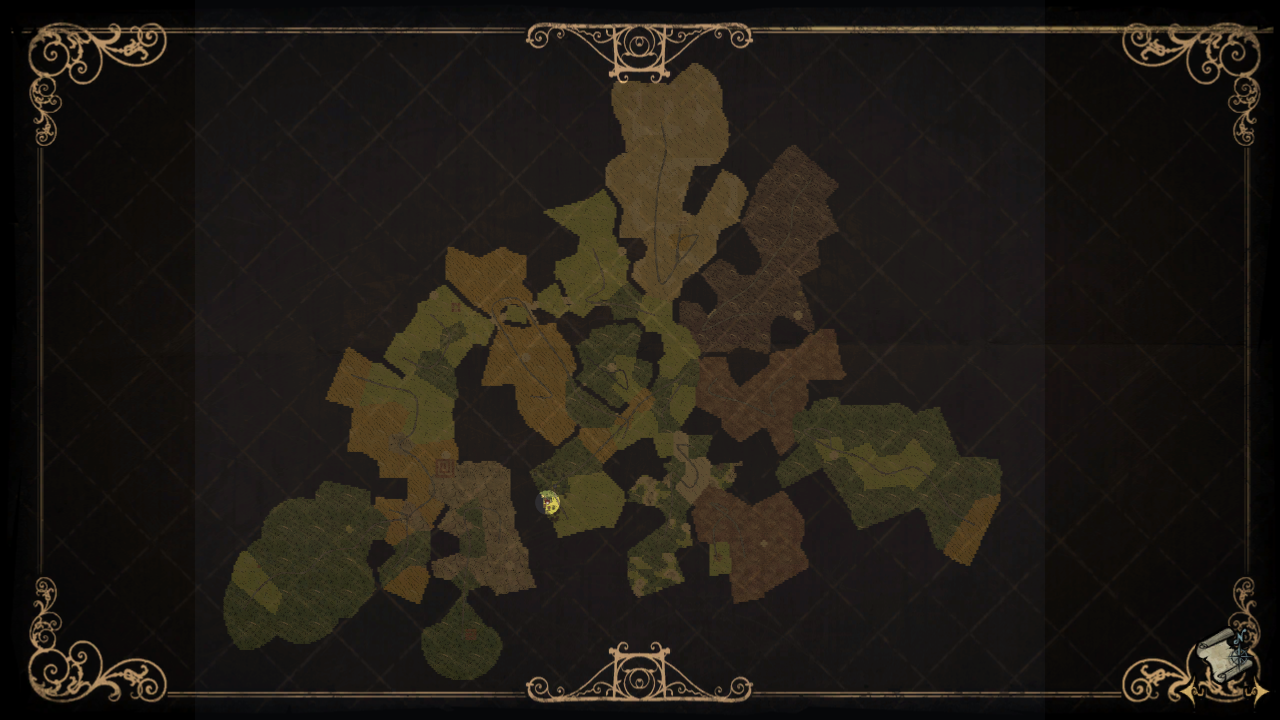
\includegraphics[width=\textwidth]{world-map}
  \caption{Example of a generated map of \ac{DST}.}
  \label{fig:world-map}
\end{figure}
As mentioned earlier, the world is procedurally generated for each game and has several different biomes that provide different kinds of resources but also dangers for the player/agent. 
We'll present and describe these biomes later on.

The world is surrounded by water and is, in many cases, composed by several peninsulas which can be composed by one or several biomes, as can be seen in Fig. \ref{fig:world-map}.
It's also common to see the formation of lakes inside the main portion of land.

During gameplay, time will pass not only in a night and day cycle but also across seasons.
The game has four seasons (Autumn, Winter, Summer, and Spring) that present different challenges during the course of the game.
In Winter the temperature descends a lot, while in Summer it rises causing the player to take damage over time due to extreme temperatures.
In Spring the rains will increase Wetness which will have the effects 
Autumn is by far the friendlier season, with mild temperatures and occasional rains, making it the perfect candidate for the starting season.

A normal world will also have caves that the players can descend to, but we will not discuss them here since we won't consider them for our agent.

Moving on to the specifics of each biome, we'll now explore a list of all the available biomes on \ac{DST} and a brief description for each of them:

\begin{itemize}
\item \textbf{Chess} this biome as an abundance of marble (a very rare material in the game), however it is protected by aggressive mobs;
\item \textbf{Deciduous Forest} being a forest, this biome is a great source of wood but also fireflies and mushrooms;
\item \textbf{Desert} can be a good source of grass and twigs (two of the most important resources on the game) but can also be very dangerous due to the Hound mob spawn points;
\item \textbf{Forest} a very good source of wood but can also contain spiders;
\item \textbf{Grassland} one of the safest biomes where the player can find a good variety of resources;
\item \textbf{Graveyard} can contain many gold nuggets and can be hazardous free.
By digging up graves the player can collect loot but there is a chance that a Ghost may spawn and attack the player.
\item \textbf{Marsh} commonly known as Swamp, is the harshest biome in the game, everything here will try and kill the player;
\item \textbf{Mosaic} this biome typically appears only once per map, and is a mix of all other biomes with not so great resources;
\item \textbf{Savanna} the abundance of grass and mobs (passive mobs like Rabbits, Birds, and Beefaloes) make this biome the best for the player to settle.
Although it can also become a dangerous place during the Beefaloes mating season where the mob becomes aggressive;
\item \textbf{Rockyland} a barren biome that contains a lot of boulders but almost nothing else. It’s a common place for Tallbirds, an aggressive mob.
\end{itemize}

For a complete listing of all the resources and where to find them, see Appendix B.

The knowledge of each of this biomes will differentiate good players from expert players, as it can strongly influence their success.
Players must know where to look what they need, where to settle, places to avoid, among others.

For the remainder of this section, we'll explore the environment of \ac{DST} which we just described in a more formal way, by looking at it from an agency point of view.

According to Russel and Norvig's (Russel and Norvig, 1995, p.46) classification of environments, \ac{DST} is a partially observable, multiagent, stochastic, episodic, dynamic, continuous, and known environment.

\begin{description}
	\item \textbf{Partially observable} In \ac{DST} the environment is actually fully observable through the scripts it natively provides to the modders and every entity is directly accessible for the agent. Despite this, we've decided to limit the observability of the environment to keep the agent in the same level of knowledge with the player, therefore, it will only have access to the same area as seen by the player in the screen.
	\item \textbf{Multiagent} Our goal is to make a social agent that plays \ac{DST}.
	As implied by the social component, there will be other agents involved. 
	In this case only a single human agent will be interacting with our agent.
	\item \textbf{Stochastic} During the game spontaneous rains can occur, meteors can fall from the skies, and even lightning strikes can set the players crops ablaze. 
	This all happens randomly and the agent will need to act accordingly in order to survive.
	\item \textbf{Episodic} Although the world is in a continuous flow and cannot really be divided into well defined episodes, we can consider it an episodic environment. 
	Due to the continuous passage of time, day after day and season after season, the player will have to overcome recurring problems, e.g. each night the player cannot stay in complete darkness because it will be attacked by Charlie (the antagonist of \ac{DST}) and each Winter the player will need to prepare itself in advance to endure the cold and the scarcity of resources.
	\item \textbf{Dynamic} During the deliberation process of the agent, the environment around him can change without direct interference from it, be it through the passing of time and therefore seasons, or be it by the aggressive and passive mobs that populate the world (e.g. Moleworms search for and eat flints, one of the most valuable resources in the game)
	\item \textbf{Continuous} In \ac{DST} time passes continuously without interruptions and even actions take time to achieve, e.g. when collecting resources there is an associated animation that must be completed for the agent to effectively receive the resources.
	\item \textbf{Known} The laws that rule \ac{DST} are all known to the agent and therefore the outcome for every action is known.
\end{description}

As described above, the world in \ac{DST} isn't a trivial one and will therefore strongly influence our decisions when devising an architecture for the agent.

Our aim is not only to build an agent that plays \ac{DST} well, but one that does it socially.
This provides a new set of challenges because the agent can't simply play the game but has to do it in a way that players won't lose interest in playing with him.
Players will also expect to engage in some sort of social activity and therefore the agent must be able to engage in this activities.

\subsection{Game play}
In order to survive the players must keep Health, Sanity and Hunger in check, as described before.
To achieve this, players must collect resources, craft weapons, tools, and equipments, fight, and find a home.
For the remainder of this section we'll explore, in a general view, what does a player do when playing \ac{DST}.
This will allow us to identify what sort of actions our agent will perform and group them into specific problems.
Before the end of the section, we'll have a comprehensive view of the problem which will allow us to better understand how can we solve it.

The first few days in \ac{DST} are the most crucial ones.
Players will usually collect flint and twigs, used in the construction of tools like axes and pickaxes, in order to collect logs (to build a fire) and gold nuggets (very important for prototyping new tools and weapons).
Finding food is of the utmost importance. 
Players usually rely on berries and carrots, which can be easily caught during the first days.
Collecting cut grass is also of the most importance given that the players will need to build traps in order to keep stockpiling food.

Along with all the collecting, players must explore the world, with the intent of finding a resource filled area where they will later set up a base camp.
Usually, by the end of the fifth day, players will have found a suitable place to build a base camp and will have found at least a gold nugget.

In the beginning, players will only have the knowledge to craft basic tools and equipment, e.g. axes, pickaxes, hammers, Grass Suits (armour), Straw Hats, among others, in a total of fifteen recipes.
By building a Science Machine, which will consume a gold nugget, players will be able to prototype new items, thus learning the recipes for them.
After prototyping a new item, players are able to freely craft that item, given that they have the required materials.
As the game progresses, players learn up to a total of over one hundred and fifty recipes.

\begin{figure}
  \centering
    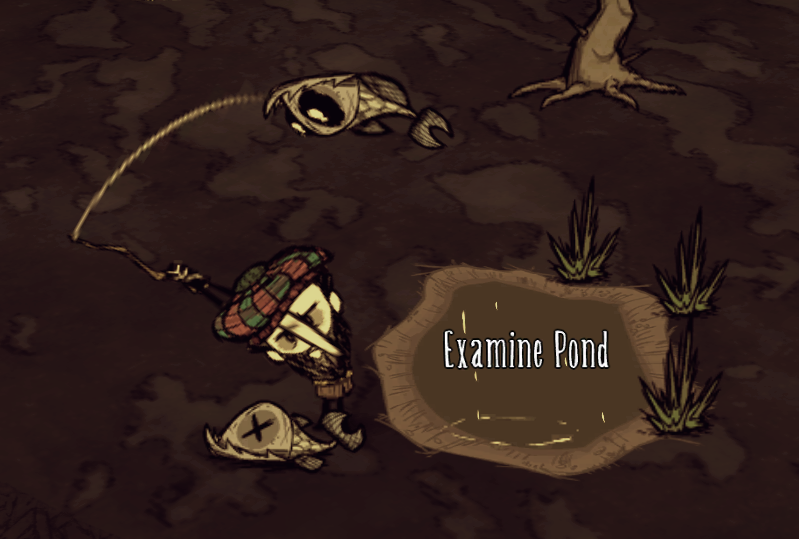
\includegraphics[width=\textwidth]{fishing}
  \caption{Wilson fishing in a Pond.}
  \label{fig:fishing}
\end{figure}

As for the base camp, players tend to find places which can provide great quantities of meat since it will be the base of the players diet after the first few days.
Rabbit holes and Ponds are usually good places, as every day they spawn Rabbit and Frogs, respectively.
Additionally, ponds can be harvested with a Fishing Rod in order to collect fishes (Fig. \ref{fig:fishing}), that once cooked in a Crock Pot will provide a good Health regenerative.
Another important factor in the choosing of a base is the proximity to manure, a must have resource for the building of farms.

As the time passes and players start to have a steady supply of food items, the tendency is to start relocating other resources to make them more accessible.
Most players will dig up Grass Tufts, Sapplings, and Berry Bushes (they provide Grass, Twigs, and Berries, respectively) and plant them near the base camp, as seen in Fig. \ref{fig:basecamp-example}.
This will greatly increase a players collecting rate as all will be concentrated in an area around the players camp, whereas the natural occurrence of such resources is usually sparse (occasionally, Berry Bushes and Grass Tufts will spawn in small clusters of nine elements near Pig Villages).
However, the relocation of Grass Tufts and Berry Bushes is usually troublesome as they require to be fertilized (using manure) in order to regrow.

\begin{figure}
  \centering
    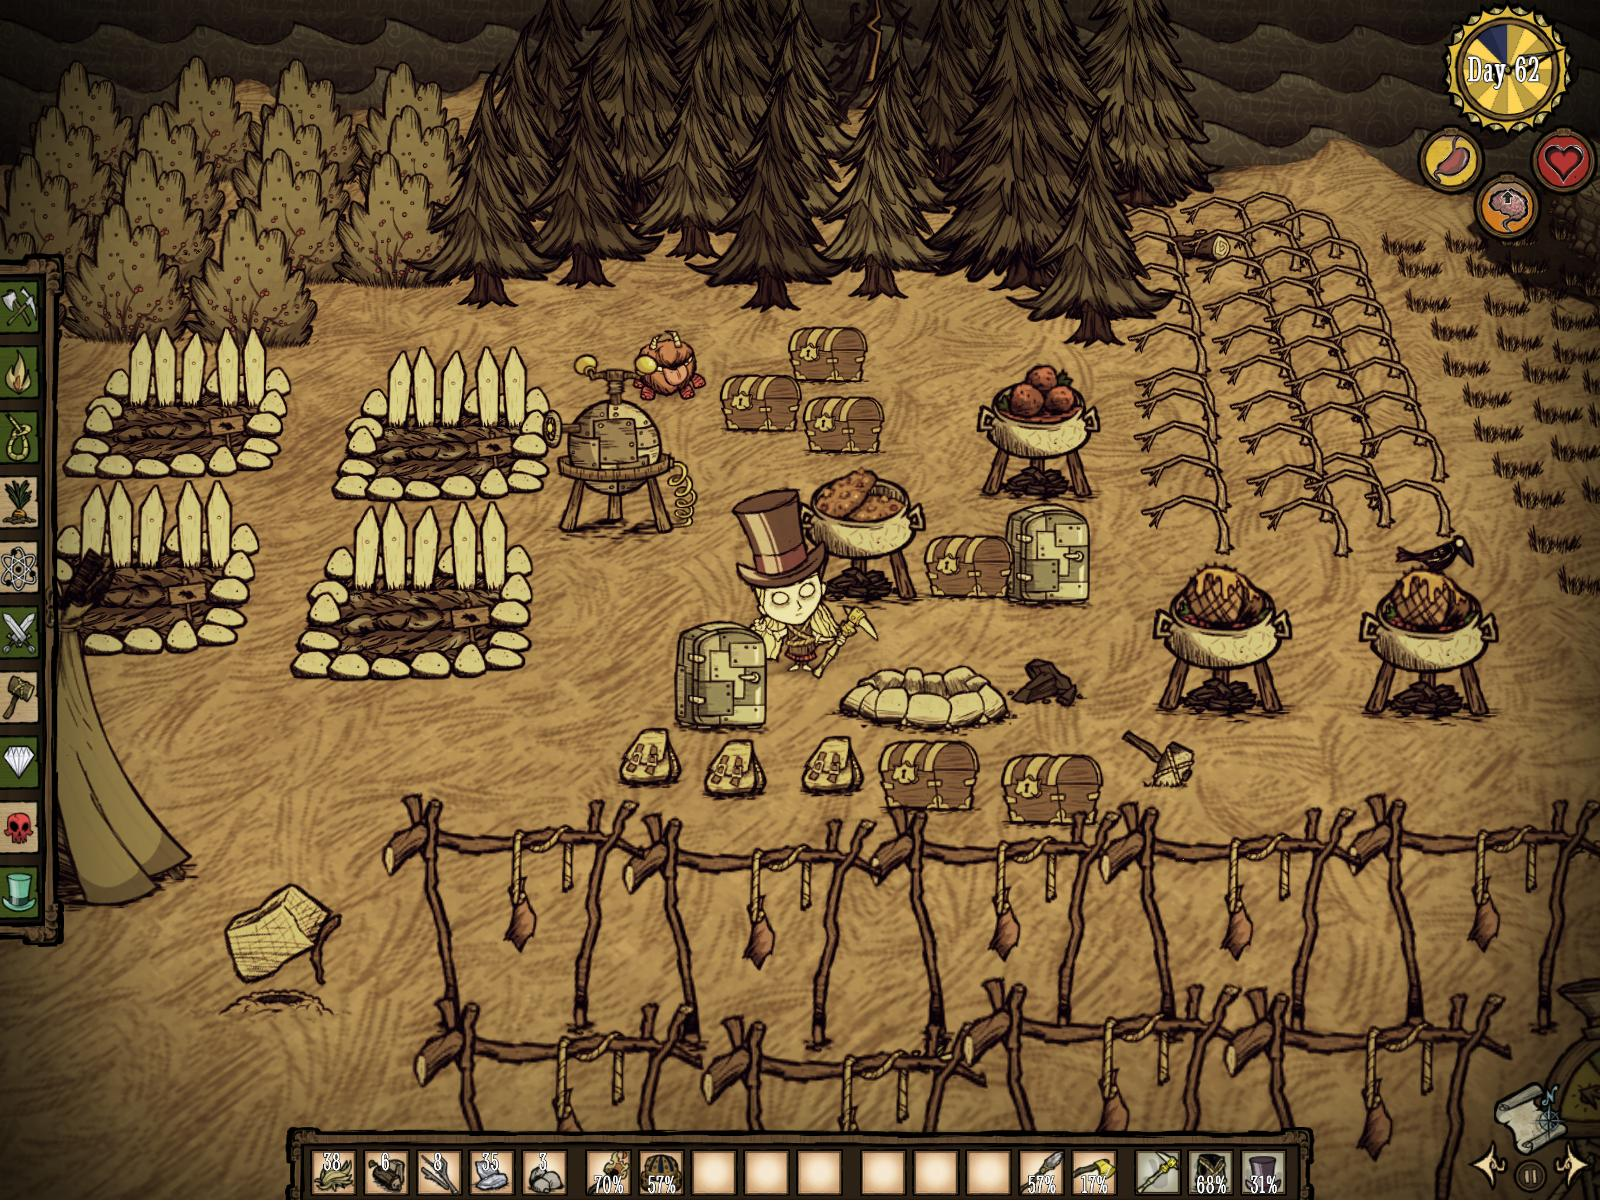
\includegraphics[width=\textwidth]{basecamp-example}
  \caption{An example of a base camp.}
  \label{fig:basecamp-example}
\end{figure}

In order to feed themselves, players use the Crock Pot to cook the food.
Crock Pots allow the elaboration of dishes that have several beneficial characteristics.
They can restore Hunger, Health and Sanity, with different dishes having different values, e.g. Fish Sticks restore a lot of Health but don't restores as much Hunger while the Meaty stew does the opposite.
For the cooking of dishes players use meats and vegetables.
The later is often obtain from farms, hence their presence in a players' base camp.

The base camp will usually be composed by a Science Machine or an Alchemy Engine (an improved version of the Science Machine), Farms, Drying Racks (used to dry meat which can them be stored for a longer period), Crock Pots, Chests (used to store items), clusters of Tress, Grass Tufts, and Saplings, and one or more Firepits.

As said before, if players stand in complete darkness for too much time, Charlie, the antagonist of the game, will attack and kill the player.
By standing next to a source of light, like a Firepit, the player avoids being attacked by Charlie.
In Winter, the Firepit will provide the player with heat in order to resist the cold which can, otherwise, kill the the player.

Now we can define which activities the player/agent engages while playing \ac{DST}.

\begin{description}
	\item \textbf{Collecting} One of the first activities in which the agent must rely upon.
This is the act by which the agent will acquire the first items that will provide him with the necessary tools to survive in the first few days of the game.
	\item \textbf{Exploring} The agent will need to explore the world in order to find every resource that it needs to survive.
	It'll also need to find a suitable place to set up a base camp.
	\item \textbf{Prototyping} Not all items will be available for Crafting or Building upon the beginning of the game.
	The agent must know that some items (the majority of them) need to be prototyped before they can be freely crafted.
	\item \textbf{Crafting} From tools to weapons and from clothes to armour, the agent will need to know all available items and its functions in order to better face the world.
	\item \textbf{Building} Similar to Crafting, but requires the player to place the structure in the world.
	\item \textbf{Fighting} The player will need to defend himself and even go on a hunt for resources.
	\item \textbf{Settling} Building up a base camp is a complex process which requires several steps.
	A good camp will help the player to survive the environment and it's hazardous conditions.
	\item \textbf{Socializing} As multi-player game, players interact with each other, either by collaborating or competing.
\end{description}
\newpage
\section{Related Work}

\subsection{Social Agents}
Agents represent a highly interdisciplinary field with influences and applications in several diverse areas such as economics, philosophy, logic, ecology, social science and computer science \cite{wooldridge:multiagent-systems}.
It's expectable that such a diverse field might have no universally accepted definition for agents \cite{wooldridge:intelligentagents}.

For the remainder of this section I'll, firstly, present a definition for what an Agent is and also see the notion of an intelligent agent.
I'll then continue on analysing what makes an agent social, thus defining Social Actions.
Finally, I'll move on into analysing some social agent's architectures.
By the end of this section it should be clear what requirements our agent must comply to in order to be called a social agent.

\subsubsection{Agents}
According to \cite{russell&norvig:aima}, an agent is "\textit{anything that can be viewed as perceiving its environment through sensors and acting upon that environment through actuators}".
Humans can be considered agents and so can computers.
We perceive our environment through our five senses (hearing, sight, touch, smell, and taste) and act upon it through our arms, hands, voice, etc. causing changes in the environment.
Computer programs perceive their environment through keystrokes, file contents, and network packets and act on the environment by displaying on the screen, writing files, and outputting music to the speakers, among many other sensors and actuators.

However there is a clear difference between a human being and a Unix daemon.
We do not usually think of Unix daemons as intelligent agents (although we might consider them agents).
As another example, even a light switch can be described as a very cooperative agent that invariably transmits electricity when we want it to do so; flicking the switch is the way we communicate our desire \cite{shoham:agentorientedprogramming}.
This example may sound absurd, but it is logical.

However, and following Shoham rationale in \cite{shoham:agentorientedprogramming}, considering the light bulb an agent, "\textit{does not buy us anything, since we essentially understand the mechanism sufficiently to have a simpler, mechanistic description of its behaviour}".
Therefore, it is important to understand what are intelligent agents and part from this general view of considering almost everything an agent.

In \cite{wooldridge:multiagent-systems}, Wooldridge identifies a list of capabilities that an intelligent agent is expected to possess.

\begin{description}
	\item[Reactivity] Intelligent agents must be able to respond in a timely fashion to changes in their environments.
	The environment may change while the agent is following a certain procedure, be it by the presence of other agents or by the characteristics of the environment.
	Blindly following that procedure without regard for environment changes is unwise as it may cause the agent to try to accomplish a goal that is no longer valid.
	\item[Proactiveness] Intelligent agents exhibit behaviours that will allow them to achieve their own goals. 
	\item[Social Ability] Intelligent agents are capable of interacting with other agents in order to achieve their goals.
\end{description}

As we can see, social ability is closely related with an intelligent agent's capabilities.

\subsubsection{What makes them Social?}
As we've seen, social ability is one of the main capabilities an agent must possess in order to be considered intelligent.
But what is Social Ability?
We can say that a social able agent performs Social Actions.

Consider a web browser: it exchanges messages with a web server through the Internet using a well-known protocol for communication, presenting web pages to the user on demand.
Can we consider a browser a social agent?

Even if we view both the browser and the web server as agents, this simple form of communication can hardly be considered social.
Going back to our example of Unix daemons, they are usually engaged in several exchanges of information with their peers and negotiate how to exchange this information, but that does not make them social.

As Castelfranchi puts it: "\textit{Agents are not 'agents' by virtue of the fact that they communicate;
they cannot be called 'social' because they communicate but the other way around: they communicate because they are social}" \cite{castelfranchi:socialactions}.

\begin{figure}
  \centering
    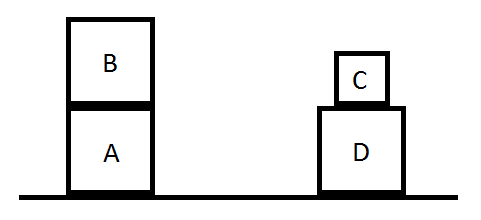
\includegraphics[width=\textwidth]{block-world-1}
  \caption{Block World initial state}
  \label{fig:block-world-1}
\end{figure}

Over the years, there as been the common misconception of considering negotiating agents as social, but as we have seen that's not always the case.
So, what makes actions social?

Imagine a block world where two agents exist, check Fig. \ref{fig:block-world-1}.
Both agents can move blocks around the world at will but cannot communicate.
The first agent, Sam, has the goal of putting both blocks A and B on the table, and the second agent, Bob, as the goal of putting block C on top of block A.
However, Bob cannot move blocks A, B, and D due to their size.
Therefore, Bob needs Sam in order to achieve its goal.

\begin{figure}
  \centering
    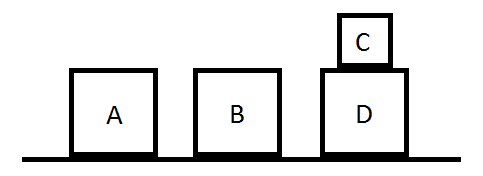
\includegraphics[width=\textwidth]{block-world-2}
  \caption{Block World after Sam's action}
  \label{fig:block-world-2}
\end{figure}

Following only its own goals, Sam will put block B on the table (check Fig. \ref{fig:block-world-2}), and Bob will then be able to put block C on top of A, completing its own goal (check Fig. \ref{fig:block-world-3}).
In this example, Sam and Bob exhibited some sort of cooperation and both achieved their own goals \footnote{This example was taken from \cite{castelfranchi:socialactions}}.

But they did so unconsciously, without knowing or having any understanding of eachother's goals, thus an action related to another agent is not necessarily social \cite{castelfranchi:individualsocialaction}.
And the opposite is also true, an action not directly related to another agent may be social in nature (consider, for example, when an agent closes a door because it doesn't want others agents looking inside the room).

\begin{figure}
  \centering
    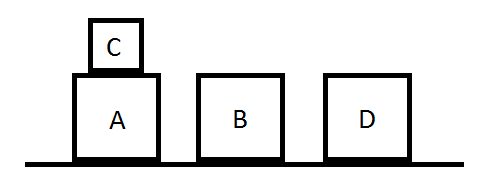
\includegraphics[width=\textwidth]{block-world-3}
  \caption{Block World final state, after Bob's action}
  \label{fig:block-world-3}
\end{figure}

To illustrate the opposite, consider two agents inside a room: the first one, John, seated at its desk and the second one, Mary, standing between John's desk and the door.
After a short conversation regarding a general topic, John, heads toward the door.
Mary, understanding John's intention of getting out of the room, promptly moves aside out of John's way, without John communicating its own intentions.

This action, of Mary stepping aside of John's way, is clearly a social one.
By interpretation of John's action, Mary demonstrated that it has an understanding of John goals and actively acts upon this knowledge.
Mary has an internal representation of John's mind, by other words, Mary is a \textit{mind-reading} agent, the basis of a social agent \cite{castelfranchi:socialactions}.

Mind-reading is the main capability an agent must posses in order to perform social actions.
And as shown in the example, this internal representation of another's agent goals and intentions, needs not be explicitly transmitted, and is, in many cases, interpreted from the agent's behaviour \cite{castelfranchi:socialactions}.

We can now understand that social agents need not only have goals and intentions of their own, but must also be able to understand and model goals and intentions of other agents.


\subsection{Modding}
Modding consists in altering an existent video game either by completely changing its gameplay experience or by changing only its visual aspect.
Some mods add new character, items, enemies, altered weapons while others only change the way the game looks, either by changing the \ac{HUD}\footnote{Heads Up Display - is a game interface used to display information to the players while in-game} or the visual effects of certain actions or items.

However there are mods that go even further by adding complete new story lines or even creating new experiences in the original games.
One of the most successful examples is the \ac{CS} mod, which completely changed Half-Life, a first person shooter action game by Valve Software.
\ac{CS} had such a success that millions of players preferred to play the mod over the original game.
Upon realising this trend, Valve Software changed it's game development and business model policies in order to include game modding as part of the gameplay experience \cite{scacchi:mods}.
More recently \ac{CS} was even released as a stand-alone game in Valve Software's popular game distributing platform, Steam.

Despite Valve Software's embrace of modding, different companies have different views on modding.
For instance, Blizzard Entertainment, publisher of World of Warcraft, one of the most played MMORPG\footnote{Massively Multi-player Online Role Playing Game} of all time; does not allow modders to change the in-game mechanics of the game, being only allowed to change the game's \ac{HUD}.

Many companies are, in certain ways, encouraging players to modify and improve their games, either by providing tools for that purpose or by providing extensive documentation.
Bethesda Softworks, Mojang, Crytek, Firaxis, Valve Software, Klei Entertainment, are some examples of such companies.
Some of them, like Klei Entertainment, maintain forums and have staff dedicated to accompany and help mod makers with their ideas and problems.

As a community driven activity (mods are made by the community, for the community), they are usually distributed through the Internet.
Several platforms provide means of distribution, being three of the most popular NexusMods\footnote{http://www.nexusmods.com}, ModDB\footnote{http://www.moddb.com}, and Steam Workshop\footnote{https://steamcommunity.com/workshop/}.
Through these platforms players can download and install mods for their favourite games or share their own creations with other players.

Survival games have followed this trend of allowing users to modify the game's content.
Notably, \ac{DST} from Klei Entertainment, has made modding a living part of the game play experience.
By subscribing to a mod in Steam's Workshop, players can experience new game play mechanics, play with different characters, craft new weapons and items, visit new in-game areas, etc., Klei Entertainment puts no barrier on what mods can do (the original game content is a mod itself).


\section{Don't Starve Together}
\ac{DST} is a multiplayer wilderness survival game developed at Klei Entertainment, where the players must survive as long as they can.
The players must face the harshnesses of a procedurally generated world that is actively trying to kill them, either by cooperating or competing with each other.
Each game can last and indefinite amount of time which is only determined by the players' ability to survive, the better you play the game, the longer you can last.

Don't Starve Together, released on April 21st of 2016, is the standalone multiplayer expansion of the uncompromising wilderness survival game Don't Starve, also released by Klei on April 23rd of 2013 (check Fig. \ref{fig:don't-starve-together-poster}).
Both titles are available in several platforms ranging from PC's to consoles and even mobile devices.
By the end of 2013 the original title (Don't Starve) sold over one million copies and, currently, there are almost 3.5 million owners of the game only on Steam.
\ac{DST} counts with over 4.6 million owners on Steam and has a daily peak of concurrent players of well over 5 thousand, reaching as high as 9 thousand concurrent players.

\begin{figure}
  \centering
    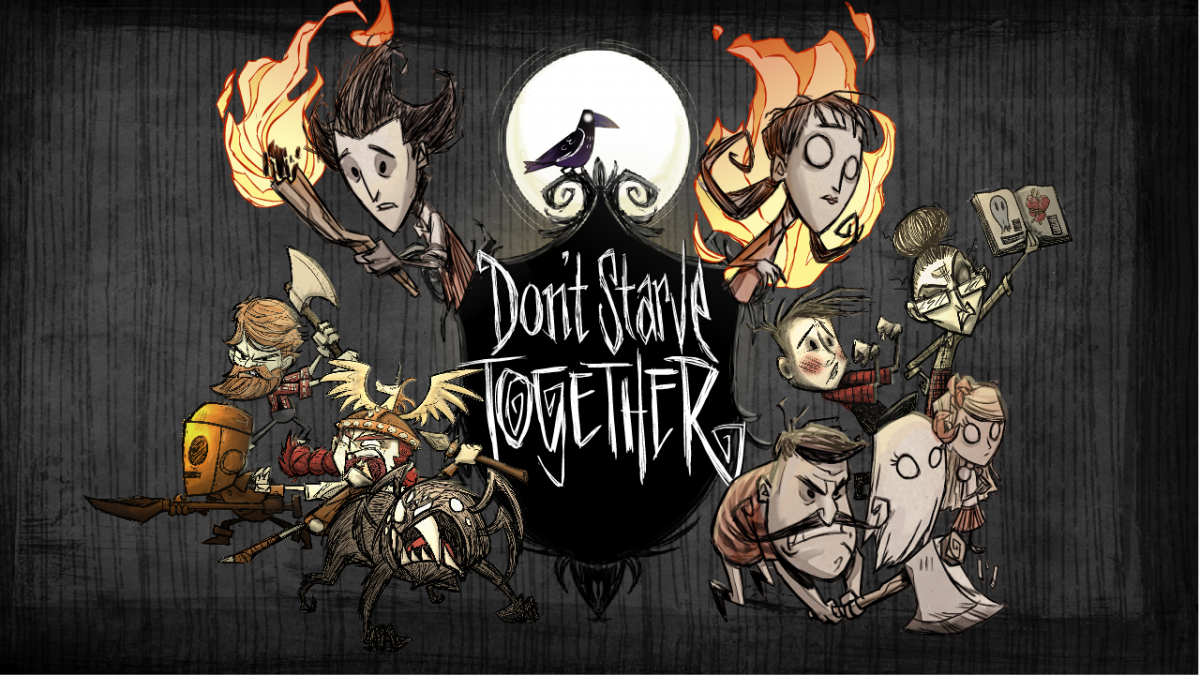
\includegraphics[width=\textwidth]{dont-starve-together-poster}
  \caption{Don't Starve Together poster with all original characters.}
  \label{fig:don't-starve-together-poster}
\end{figure}

The game counts with a developer maintained forum where there is an active participation in the forums by Klei Entertainment staff, which help in problem solving for community developed mods, bug fixing the game, and sharing development notes on the game.
Over twenty-five hundred mods are available for the game on the Steam Workshop, making \ac{DST} a well-suited option to implement and test our solution.

\subsection{The Game}
Before playing \ac{DST}, the players must first choose a character from a list of different characters.
Different characters have different characteristics and may be affected by the world in different ways (for example, WX-78 can eat spoiled food without penalties) and can even possess special items (such as Woodie's axe, \textit{Lucy the Axe}).
Upon entering the world, the player has nothing in its inventory (except for character specific items, as referred earlier) and thus needs to start collecting resources in order to survive.

During the game the player must pay attention to the three characteristics of his character: Hunger, Sanity, and Health.
The player dies (in \ac{DST} the player actually becomes a ghost that can be revived by other players or by finding a Touch Stone) once his Health reaches zero.
Both Hunger and Sanity can cause the player to loose Health (Sanity doesn't directly cause the player to loose Health, but the player will be attacked by creatures that appear due to the character's paranoia).

So, it is important for the player to keep Hunger, Sanity, and Health in check in order to survive.
The player will also need to take attention to the character's Wetness which is caused by rains.
Wetness will cause the items to loose efficiency and by using wet items the character will lose Sanity over time.
The player must also be aware of the temperature of his character as it can cause damage.
Both extreme hot and extreme cold will cause the player to continuously loose Health.

Taking care of the character's Hunger, Sanity, and Health is the players main concern during game play.
The player will accomplish this by collecting resources, crafting new items, cooking food, among other things (we will explore the player's possible actions in full detail further on).

\subsection{The World}

\begin{figure}
  \centering
    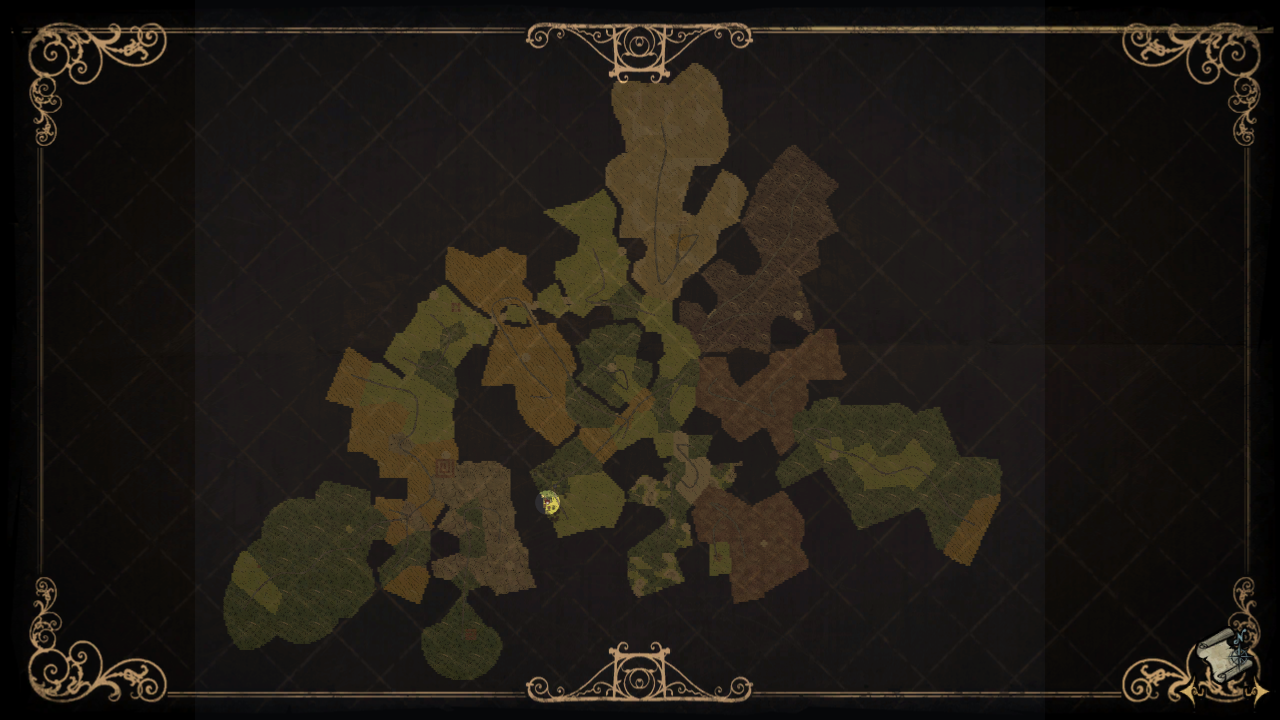
\includegraphics[width=\textwidth]{world-map}
  \caption{Example of a generated map of \ac{DST}.}
  \label{fig:world-map}
\end{figure}
As mentioned earlier, the world is procedurally generated for each game and has several different biomes that provide different kinds of resources but also dangers for the player/agent. 
We'll present and describe these biomes later on.

The world is surrounded by water and is, in many cases, composed by several peninsulas which can be composed by one or several biomes, as can be seen in Fig. \ref{fig:world-map}.
It's also common to see the formation of lakes inside the main portion of land.

During gameplay, time will pass not only in a night and day cycle but also across seasons.
The game has four seasons (Autumn, Winter, Summer, and Spring) that present different challenges during the course of the game.
In Winter the temperature descends a lot, while in Summer it rises causing the player to take damage over time due to extreme temperatures.
In Spring the rains will increase Wetness which will have the effects 
Autumn is by far the friendlier season, with mild temperatures and occasional rains, making it the perfect candidate for the starting season.

A normal world will also have caves that the players can descend to, but we will not discuss them here since we won't consider them for our agent.

Moving on to the specifics of each biome, we'll now explore a list of all the available biomes on \ac{DST} and a brief description for each of them:

\begin{itemize}
\item \textbf{Chess} this biome as an abundance of marble (a very rare material in the game), however it is protected by aggressive mobs;
\item \textbf{Deciduous Forest} being a forest, this biome is a great source of wood but also fireflies and mushrooms;
\item \textbf{Desert} can be a good source of grass and twigs (two of the most important resources on the game) but can also be very dangerous due to the Hound mob spawn points;
\item \textbf{Forest} a very good source of wood but can also contain spiders;
\item \textbf{Grassland} one of the safest biomes where the player can find a good variety of resources;
\item \textbf{Graveyard} can contain many gold nuggets and can be hazardous free.
By digging up graves the player can collect loot but there is a chance that a Ghost may spawn and attack the player.
\item \textbf{Marsh} commonly known as Swamp, is the harshest biome in the game, everything here will try and kill the player;
\item \textbf{Mosaic} this biome typically appears only once per map, and is a mix of all other biomes with not so great resources;
\item \textbf{Savanna} the abundance of grass and mobs (passive mobs like Rabbits, Birds, and Beefaloes) make this biome the best for the player to settle.
Although it can also become a dangerous place during the Beefaloes mating season where the mob becomes aggressive;
\item \textbf{Rockyland} a barren biome that contains a lot of boulders but almost nothing else. It’s a common place for Tallbirds, an aggressive mob.
\end{itemize}

For a complete listing of all the resources and where to find them, see Appendix B.

The knowledge of each of this biomes will differentiate good players from expert players, as it can strongly influence their success.
Players must know where to look what they need, where to settle, places to avoid, among others.

For the remainder of this section, we'll explore the environment of \ac{DST} which we just described in a more formal way, by looking at it from an agency point of view.

According to Russel and Norvig's (Russel and Norvig, 1995, p.46) classification of environments, \ac{DST} is a partially observable, multiagent, stochastic, episodic, dynamic, continuous, and known environment.

\begin{description}
	\item \textbf{Partially observable} In \ac{DST} the environment is actually fully observable through the scripts it natively provides to the modders and every entity is directly accessible for the agent. Despite this, we've decided to limit the observability of the environment to keep the agent in the same level of knowledge with the player, therefore, it will only have access to the same area as seen by the player in the screen.
	\item \textbf{Multiagent} Our goal is to make a social agent that plays \ac{DST}.
	As implied by the social component, there will be other agents involved. 
	In this case only a single human agent will be interacting with our agent.
	\item \textbf{Stochastic} During the game spontaneous rains can occur, meteors can fall from the skies, and even lightning strikes can set the players crops ablaze. 
	This all happens randomly and the agent will need to act accordingly in order to survive.
	\item \textbf{Episodic} Although the world is in a continuous flow and cannot really be divided into well defined episodes, we can consider it an episodic environment. 
	Due to the continuous passage of time, day after day and season after season, the player will have to overcome recurring problems, e.g. each night the player cannot stay in complete darkness because it will be attacked by Charlie (the antagonist of \ac{DST}) and each Winter the player will need to prepare itself in advance to endure the cold and the scarcity of resources.
	\item \textbf{Dynamic} During the deliberation process of the agent, the environment around him can change without direct interference from it, be it through the passing of time and therefore seasons, or be it by the aggressive and passive mobs that populate the world (e.g. Moleworms search for and eat flints, one of the most valuable resources in the game)
	\item \textbf{Continuous} In \ac{DST} time passes continuously without interruptions and even actions take time to achieve, e.g. when collecting resources there is an associated animation that must be completed for the agent to effectively receive the resources.
	\item \textbf{Known} The laws that rule \ac{DST} are all known to the agent and therefore the outcome for every action is known.
\end{description}

As described above, the world in \ac{DST} isn't a trivial one and will therefore strongly influence our decisions when devising an architecture for the agent.

Our aim is not only to build an agent that plays \ac{DST} well, but one that does it socially.
This provides a new set of challenges because the agent can't simply play the game but has to do it in a way that players won't lose interest in playing with him.
Players will also expect to engage in some sort of social activity and therefore the agent must be able to engage in this activities.

\subsection{Game play}
In order to survive the players must keep Health, Sanity and Hunger in check, as described before.
To achieve this, players must collect resources, craft weapons, tools, and equipments, fight, and find a home.
For the remainder of this section we'll explore, in a general view, what does a player do when playing \ac{DST}.
This will allow us to identify what sort of actions our agent will perform and group them into specific problems.
Before the end of the section, we'll have a comprehensive view of the problem which will allow us to better understand how can we solve it.

The first few days in \ac{DST} are the most crucial ones.
Players will usually collect flint and twigs, used in the construction of tools like axes and pickaxes, in order to collect logs (to build a fire) and gold nuggets (very important for prototyping new tools and weapons).
Finding food is of the utmost importance. 
Players usually rely on berries and carrots, which can be easily caught during the first days.
Collecting cut grass is also of the most importance given that the players will need to build traps in order to keep stockpiling food.

Along with all the collecting, players must explore the world, with the intent of finding a resource filled area where they will later set up a base camp.
Usually, by the end of the fifth day, players will have found a suitable place to build a base camp and will have found at least a gold nugget.

In the beginning, players will only have the knowledge to craft basic tools and equipment, e.g. axes, pickaxes, hammers, Grass Suits (armour), Straw Hats, among others, in a total of fifteen recipes.
By building a Science Machine, which will consume a gold nugget, players will be able to prototype new items, thus learning the recipes for them.
After prototyping a new item, players are able to freely craft that item, given that they have the required materials.
As the game progresses, players learn up to a total of over one hundred and fifty recipes.

\begin{figure}
  \centering
    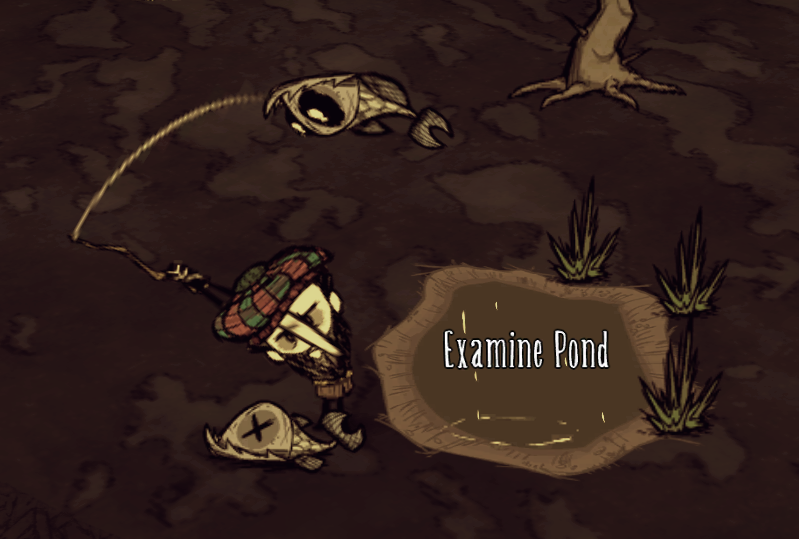
\includegraphics[width=\textwidth]{fishing}
  \caption{Wilson fishing in a Pond.}
  \label{fig:fishing}
\end{figure}

As for the base camp, players tend to find places which can provide great quantities of meat since it will be the base of the players diet after the first few days.
Rabbit holes and Ponds are usually good places, as every day they spawn Rabbit and Frogs, respectively.
Additionally, ponds can be harvested with a Fishing Rod in order to collect fishes (Fig. \ref{fig:fishing}), that once cooked in a Crock Pot will provide a good Health regenerative.
Another important factor in the choosing of a base is the proximity to manure, a must have resource for the building of farms.

As the time passes and players start to have a steady supply of food items, the tendency is to start relocating other resources to make them more accessible.
Most players will dig up Grass Tufts, Sapplings, and Berry Bushes (they provide Grass, Twigs, and Berries, respectively) and plant them near the base camp, as seen in Fig. \ref{fig:basecamp-example}.
This will greatly increase a players collecting rate as all will be concentrated in an area around the players camp, whereas the natural occurrence of such resources is usually sparse (occasionally, Berry Bushes and Grass Tufts will spawn in small clusters of nine elements near Pig Villages).
However, the relocation of Grass Tufts and Berry Bushes is usually troublesome as they require to be fertilized (using manure) in order to regrow.

\begin{figure}
  \centering
    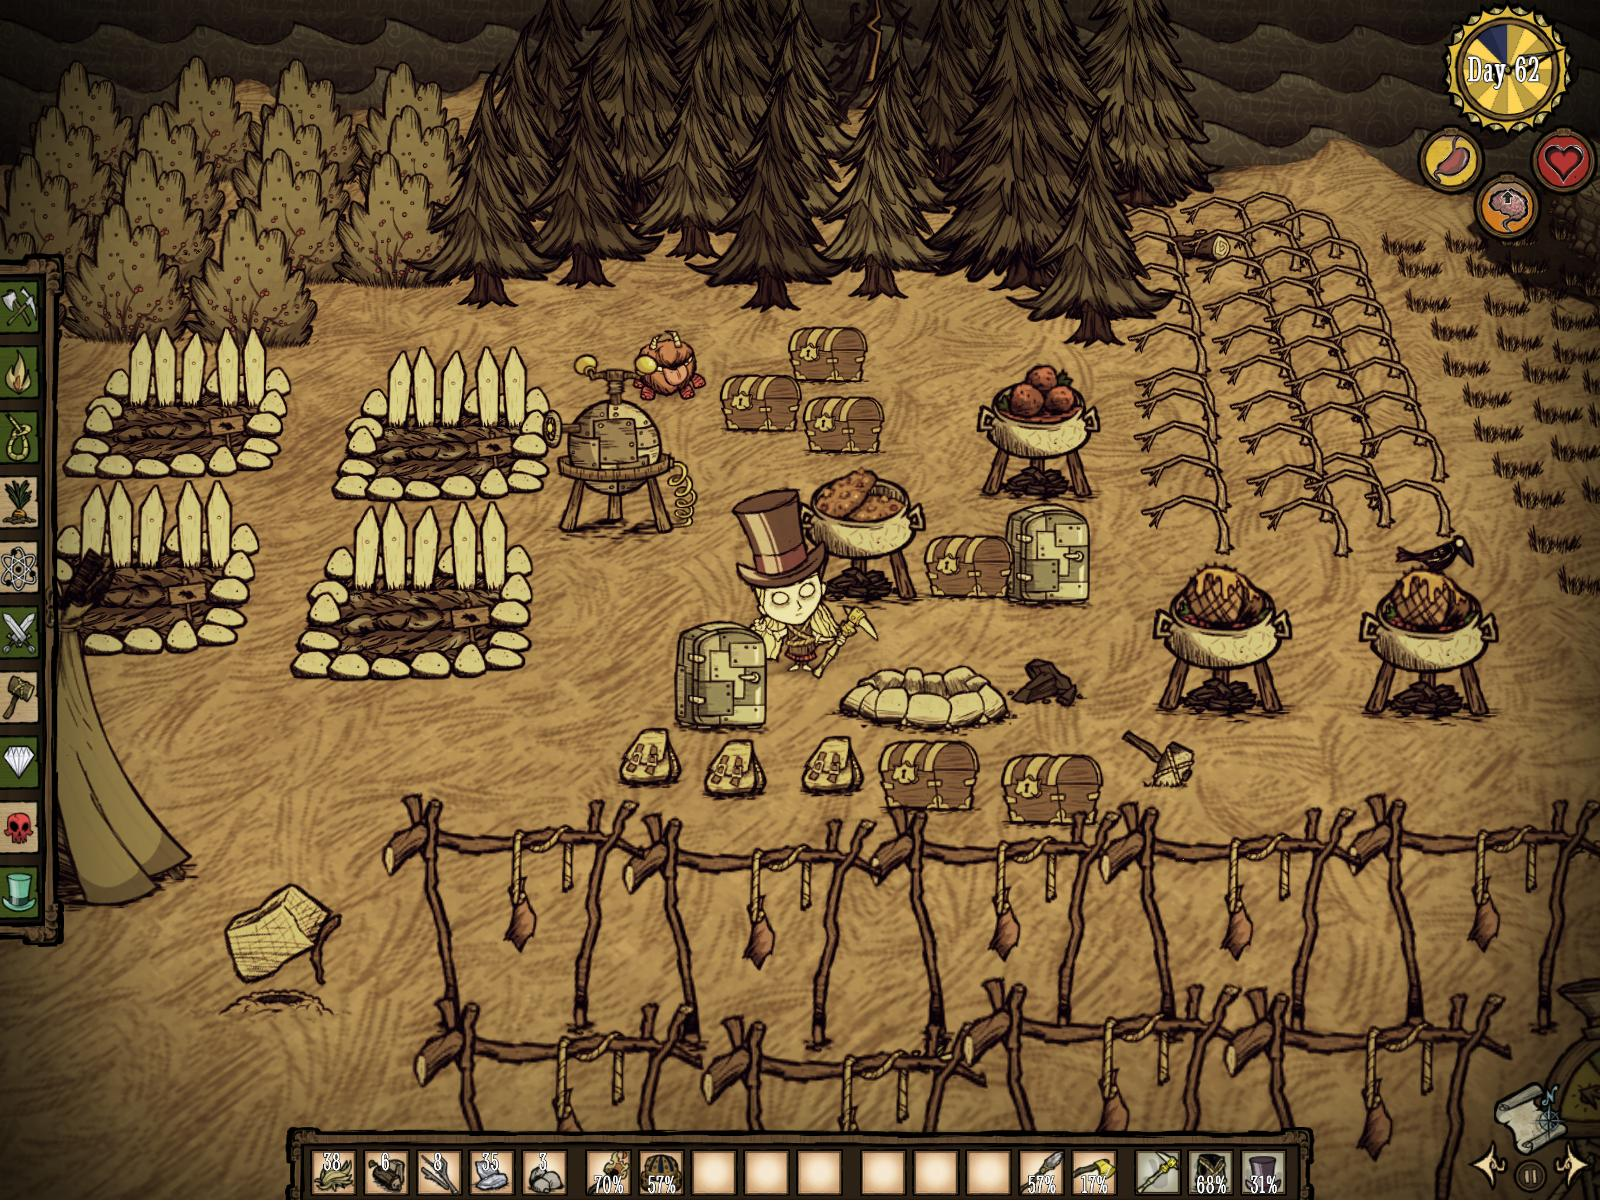
\includegraphics[width=\textwidth]{basecamp-example}
  \caption{An example of a base camp.}
  \label{fig:basecamp-example}
\end{figure}

In order to feed themselves, players use the Crock Pot to cook the food.
Crock Pots allow the elaboration of dishes that have several beneficial characteristics.
They can restore Hunger, Health and Sanity, with different dishes having different values, e.g. Fish Sticks restore a lot of Health but don't restores as much Hunger while the Meaty stew does the opposite.
For the cooking of dishes players use meats and vegetables.
The later is often obtain from farms, hence their presence in a players' base camp.

The base camp will usually be composed by a Science Machine or an Alchemy Engine (an improved version of the Science Machine), Farms, Drying Racks (used to dry meat which can them be stored for a longer period), Crock Pots, Chests (used to store items), clusters of Tress, Grass Tufts, and Saplings, and one or more Firepits.

As said before, if players stand in complete darkness for too much time, Charlie, the antagonist of the game, will attack and kill the player.
By standing next to a source of light, like a Firepit, the player avoids being attacked by Charlie.
In Winter, the Firepit will provide the player with heat in order to resist the cold which can, otherwise, kill the the player.

Now we can define which activities the player/agent engages while playing \ac{DST}.

\begin{description}
	\item \textbf{Collecting} One of the first activities in which the agent must rely upon.
This is the act by which the agent will acquire the first items that will provide him with the necessary tools to survive in the first few days of the game.
	\item \textbf{Exploring} The agent will need to explore the world in order to find every resource that it needs to survive.
	It'll also need to find a suitable place to set up a base camp.
	\item \textbf{Prototyping} Not all items will be available for Crafting or Building upon the beginning of the game.
	The agent must know that some items (the majority of them) need to be prototyped before they can be freely crafted.
	\item \textbf{Crafting} From tools to weapons and from clothes to armour, the agent will need to know all available items and its functions in order to better face the world.
	\item \textbf{Building} Similar to Crafting, but requires the player to place the structure in the world.
	\item \textbf{Fighting} The player will need to defend himself and even go on a hunt for resources.
	\item \textbf{Settling} Building up a base camp is a complex process which requires several steps.
	A good camp will help the player to survive the environment and it's hazardous conditions.
	\item \textbf{Socializing} As multi-player game, players interact with each other, either by collaborating or competing.
\end{description}


\subsection{Discussion}

Bearing in mind the objectives of this work, modding represents a suitable medium by which we can implement and test our agent.
\ac{DST} appears as a good candidate for such work.
\newpage
\section{Solution Proposal}

\subsection{Approach}

\subsection{Architecture}

\subsection{Evaluation}

\subsection{Planning}
\newpage
\printbibliography
\newpage
\addcontentsline{toc}{section}{Appendix A -- List of Acronyms}
\section*{Appendix A -- List of Acronyms}
\begin{acronym}
\acro{AI}{Artificial Intelligence}
\acro{DST}{Don't Starve Together}
\acro{CS}{Counter Strike}
\acro{HUD}{Heads Up Display}
\acro{NPC}{Non Playable Character}
\end{acronym}

\end{document}